% ---------------------------- Preamble starts here ----------------------------

\documentclass[aspectratio=169]{beamer} %Remove [aspectratio=169] to get non-wide 4:3 slide aspect ratio

%-----------------------------------------------
% --- Set beamer theme
\usetheme{Metropolis}
\setbeamertemplate{footline}{}				% Remove automatic footer
\setbeamertemplate{navigation symbols}{}	% Comment this line to display navigation symbols

%-----------------------------------------------
% Load i2i symbol
\addtobeamertemplate{frametitle}{}{%
\begin{textblock*}{\linewidth}(0cm,7.4cm) % Replace with (0cm, 8cm) if using non-wide slide aspect
	
\includegraphics[width=\linewidth]{img/Footer.png}
\end{textblock*}}

\setbeamertemplate{footline}{\hfill\insertframenumber/\inserttotalframenumber}

%-----------------------------------------------
% --- Load packages
\usepackage{textpos}		% To align objects correctly
\usepackage{multicol}		% To right in multiple columns
\usepackage{color}			% To color text

\definecolor{links}{HTML}{2A1B81}
\hypersetup{colorlinks,linkcolor=,urlcolor=links}

%-----------------------------------------------
% --- Include link to last commit
\usepackage{xstring}
\usepackage{catchfile}

%Set this user input
\newcommand{\gitfolder}{../../../../.git} %relative path to .git folder from .tex doc
\newcommand{\reponame}{worldbank/dime-github-trainings} % Name of account and repo be set in URL

%Based on this https://tex.stackexchange.com/questions/455396/how-to-include-the-current-git-commit-id-and-branch-in-my-document
\CatchFileDef{\headfull}{\gitfolder/HEAD.}{} 				%Get path to head file for checked out branch
\StrGobbleRight{\headfull}{1}[\head]						%Remove end of line character
\StrBehind[2]{\head}{/}[\branch]							%Parse out the path only
\CatchFileDef{\commit}{\gitfolder/refs/heads/\branch.}{}	%Get the content of the branch head
\StrGobbleRight{\commit}{1}[\commithash]					%Remove end of line characted

%Build the URL to this commit based on the information we now have
\newcommand{\commiturl}{\url{https://github.com/\reponame/commit/\commithash}}

%-----------------------------------------------
% --- Add your information here
\title{WB AWS Onboarding - WB AWS Tutorial}
\author{DIME Analytics}
\institute{DIME - The World Bank - \trainingURL{https://www.worldbank.org/en/research/dime}}
\date{\today}

\newcommand{\trainingURL}[1]{{\color{blue}\url{#1}}}

\newcommand{\trainerEmail}{\trainingURL{kbjarkefur@worldbank.org} }

\newcommand{\teamName}{DeJure }
\newcommand{\ectwoName}{walxpdimekt01}
\newcommand{\srvAcctName}{srvdimeieconnect}

% ---------------------------- Preamble ends here ----------------------------

\begin{document}

\begin{frame}
	\frametitle{Prerequisites}

		To follow all steps in this presentation you need:

		\begin{itemize}
			\setlength\itemsep{.8em}
			\item A WB managed computer, for example:
			\begin{itemize}
				\item A WB laptop or desktop
				\item A remote connection to a WB laptop or desktop
				\item A Dedicated WB VDI (virtual desktop) - a Regular VDI is not sufficient
			\end{itemize}
			\item A WB SecureID token
			\item PuTTY installed on the WB computer - self install through ``Software Center''
			\item A WB C-account - see set-up instructions in Part 2
			\item The \textit{Microsoft Authenticator} app - see set-up instructions in Part 2
		\end{itemize}
\end{frame}

\begin{frame}
	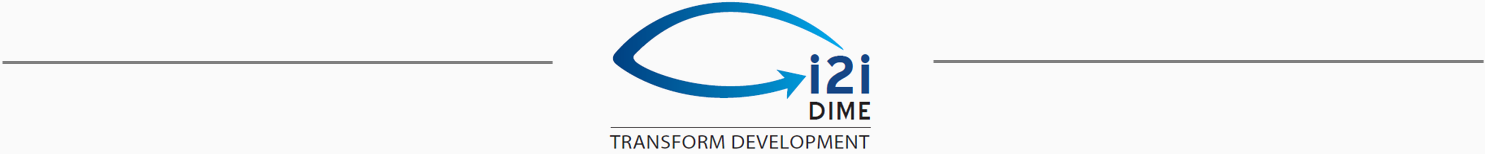
\includegraphics[width=\textwidth]{img/Header.png}
	\vspace{-0.2cm}
	\titlepage 	 % Opening slide, prints inform
\end{frame}

\begin{frame}
	\frametitle{Outline}

	\begin{columns}[c]
		\column{.65\textwidth} % Left column and width
		\Huge Outline of presentation:
		\vspace{.7cm}\newline
		\large \textbf{Part 1:} AWS WB Island and best practices
		\vspace{.7cm}\newline
		\large \textbf{Part 2:} Browser access - WB AWS resources
		\vspace{.7cm}\newline
		\large \textbf{Part 3:} Command line access - WB AWS resources

	\end{columns}
\end{frame}

\section{Part 1: AWS WB Island and AWS best practices}

\begin{frame}
\frametitle{How are WB AWS resources set-up}

	\begin{columns}[c]
		\column{.50\textwidth} % Left column and width
		\large All WB AWS resources will be hosted in a
		VPC (Virtual Private Cloud) - 
		called \textbf{AWS Island} in this presentation
		\vspace{.3cm}\newline
		\large All traffic to and from any resource in
		the AWS Island goes through the gateway (gw) server,
		where all security setting are set-up.
		\vspace{.3cm}\newline
		\large This means that 
		it is easier to connect resources within the island and
		your resources only need simplified security settings

		\column{.50\textwidth} % Right column and width
		\begin{figure}
			\centering
			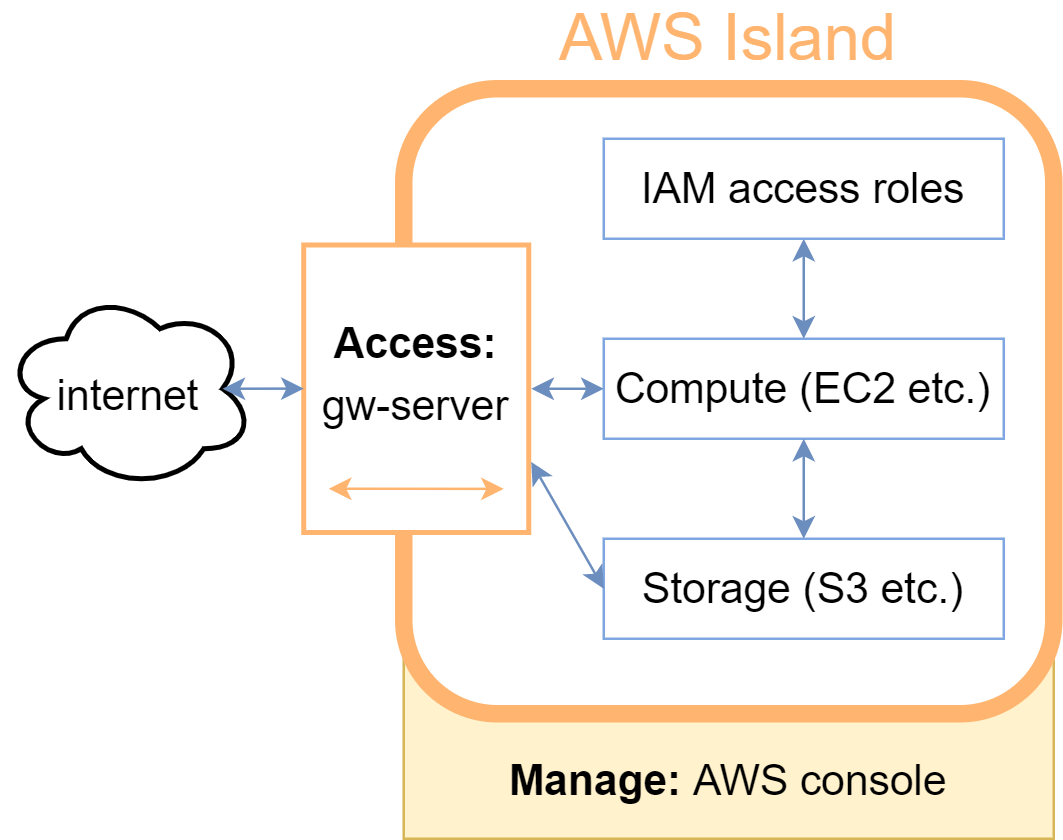
\includegraphics[width=\textwidth]{./img/wb-aws.png}
		\end{figure}

	\end{columns}
\end{frame}

\begin{frame}
	\frametitle{How to access a resource}
	
	\begin{columns}[c]
		\column{.50\textwidth} % Left column and width
		\large There are two methods to access your resource - many tasks can be done using both methods
		\vspace{.3cm}\newline
		\large \textbf{Browser access} (Part 2): This is typically used to start/stop EC2 instances and manually upload files to S3 buckets
		\vspace{.3cm}\newline
		\large \textbf{Command line access} (Part 3): This is typically used to execute scripts on an EC2 server, or upload large amounts of files to S3 buckets
		
		\column{.50\textwidth} % Right column and width
		\begin{figure}
			\centering
			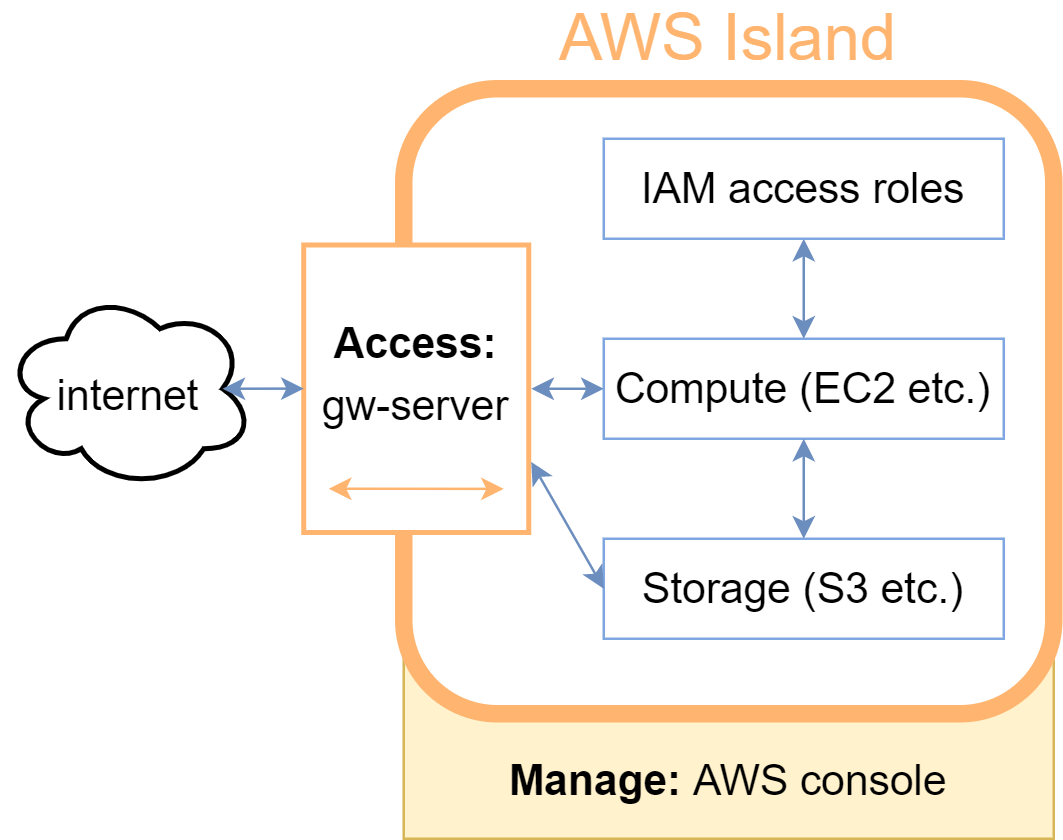
\includegraphics[width=\textwidth]{./img/wb-aws.png}
		\end{figure}
		
	\end{columns}
\end{frame}


\begin{frame}
	\frametitle{Best practice: EC2 cost efficiency - auto-stop}

	\begin{columns}[c]

		\column{.05\textwidth} % Right column and width

		\column{.55\textwidth} % Left column and width
		\textbf{If using EC2 instances:}
		
		\vspace{.5cm}
		
		Not stopping an instance when you are not running a script,
		is like making an international phone call once per week,
		and not hanging up the phone between the calls
		- it will be very expensive.

		\vspace{.5cm}

		When possible we will always enable \textbf{auto-stop},
		so that when the CPU of the instance has,
		for example, been under 5\% for over 30 min the instance
		automatically shuts down until manually restarted.

		\column{.1\textwidth} % Right column and width

		\column{.25\textwidth} % Right column and width
		\begin{figure}
			\centering
			
\includegraphics[width=\textwidth]{./img/international-call.png}
		\end{figure}

		\column{.05\textwidth} % Right column and width
	\end{columns}
\end{frame}

\begin{frame}
	\frametitle{Best practice: EC2 cost efficiency - EC2 is not a code editor}

	\begin{columns}[c]

		\column{.55\textwidth} % Left column and width
		It is cost prohibitive to use a cloud resource as code editors!

		\vspace{.5cm}

		Only already tested code should run in the cloud
		- exceptions are small fixes like broken file paths etc.

		\vspace{.5cm}

		DIME Analytics can help you set up a workflow
		where code is developed on a sample locally, 
		pushed to the cloud resource using Git,
		and only tested version of the code runs in the cloud.

		\column{.45\textwidth} % Right column and width
		\begin{figure}
			\centering
			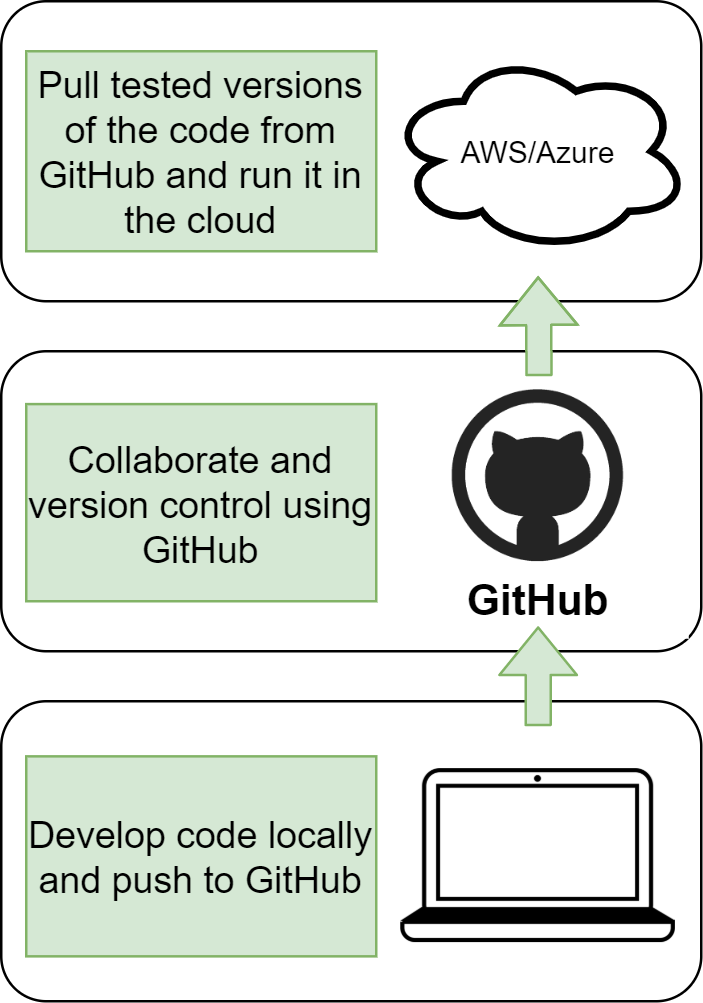
\includegraphics[width=.8\textwidth]{./img/code-workflow.png}
		\end{figure}
	\end{columns}
\end{frame}

\begin{frame}
	\frametitle{Cloud Storage}

	Where will data be stored? Storage is often cheap in the cloud,
	but not all options are cheap.
	All EC2 instances come with some EBS storage where,
	for example, Python libraries, NLP corpora,  GitHub clones, etc. are saved
	\vspace{-.5cm}
	\begin{table}
		\begin{tabular}{p{0.12\textwidth}p{0.88\textwidth}}
			Service & Pros and Cons\\
			\hline \hline
			\textbf{S3} & Typically used to store data in file format (\textit{.csv}, etc.).
			Cheap and you only pay for what you actually use
			- requires specific code libraries to access files\\[.2cm]
			\textbf{EBS} & The EBS storage can be expanded so you can store data there as well.
			EBS is more expensive per GB and you pay for capacity whether you use it or not.
			Suitable when data must be stored in the same drive as the code.\\[.2cm]
			\textbf{Databases} & All types of DBs are available in AWS.
			DBs can be more expensive than S3 but are queried faster
			- good for dashboards
		\end{tabular}
	\end{table}
\end{frame}

\section{Part 2: Browser access - WB AWS resources}

\begin{frame}
	\frametitle{WB AWS management console}
	\begin{columns}[c]
		\column{.50\textwidth} % Left column and width
		We manage the settings of our AWS resources by accessing the \textbf{AWS management console} using a web browser
		\vspace{.5cm}\newline
		Most settings are only available to ITS, but a few management console features are important to us, examples include:
		\begin{itemize}
			%\setlength\itemsep{1em}
			\item Start and stop EC2 instances (cost efficiency)
			\item Manually upload files to S3 buckets
		\end{itemize}

		\column{.50\textwidth} % Right column and width
		\begin{figure}
			\centering
			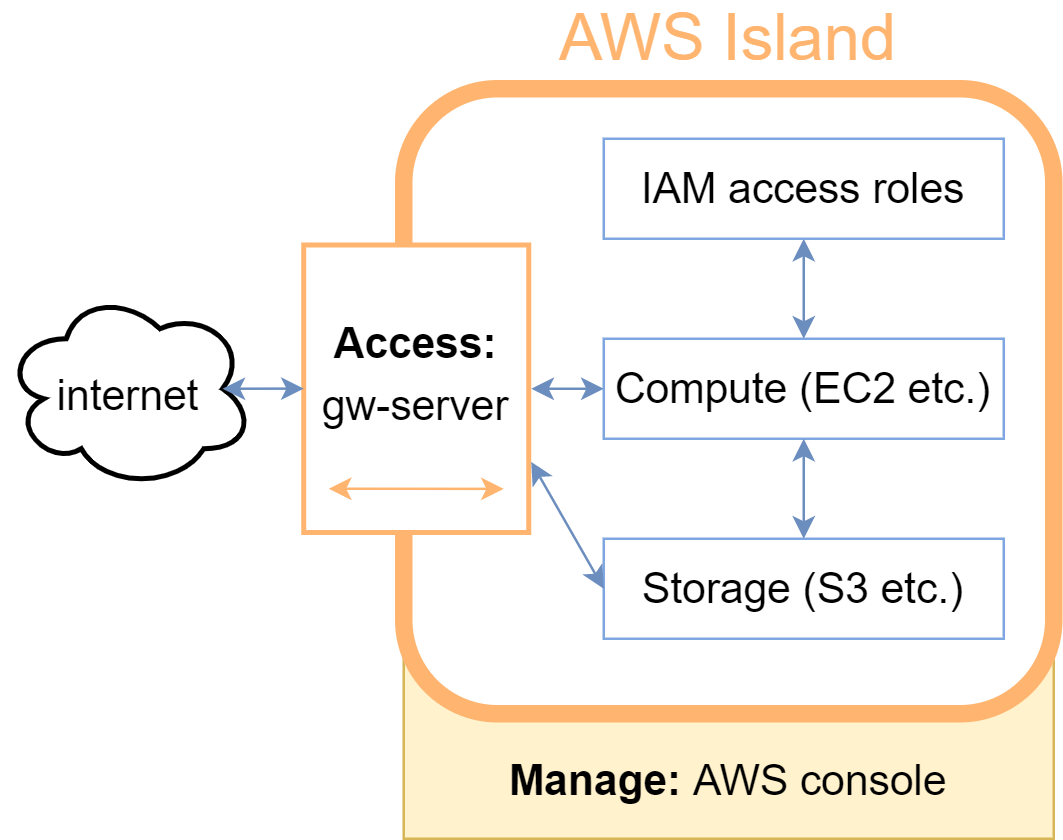
\includegraphics[width=\textwidth]{./img/wb-aws.png}
		\end{figure}

	\end{columns}
\end{frame}

\begin{frame}
	\frametitle{WB AWS management console - set-up}
	\begin{columns}[c]
		
		\column{.80\textwidth} % Right column and width
		
		\textbf{Set-up:} The set-up steps only has to be done the first time you access the AWS management console

	\end{columns}
\end{frame}


\begin{frame}
	\frametitle{WB AWS management console - set-up (1/2)}
	\begin{columns}[c]

		\column{.60\textwidth} % Right column and width

		To access the AWS management console we need a \textit{C-account} - C as in cloud

		\begin{enumerate}
			\item Request C-account on eServices 
			- (search for "\textit{C Account Request}")
			\item Wait for the request to be completed
			\item Reset auto-generated C-account password:
			\begin{enumerate}
				\item Go to \textit{http://password/} on WB intranet
				\item Log in using SecureID and select \textit{Manage Passwords}
				\item Click \textit{Change} for your \textit{C$<$UPI$>$} account
			\end{enumerate}
			\item Add this password to your password manager!
		\end{enumerate}

		\column{.40\textwidth} % Right column and width
		\begin{figure}
			\centering
			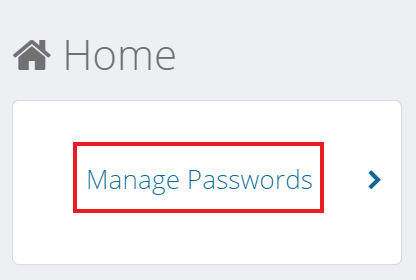
\includegraphics[width=.5\textwidth]{./img/password-1.png}
		\end{figure}
		\vspace{.2cm}
		\begin{figure}
			\centering
			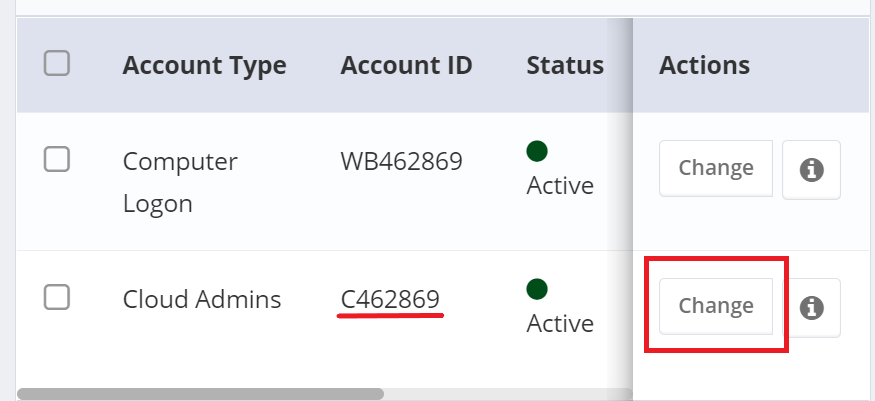
\includegraphics[width=1\textwidth]{./img/password-2.png}
		\end{figure}

	\end{columns}
\end{frame}

\begin{frame}
	\frametitle{WB AWS management console - set-up (2/2)}
	\begin{columns}[c]

		\column{.650\textwidth} % Right column and width

		\begin{enumerate}
			\item Download the \textit{Microsoft Authenticator} app to your smartphone
			\item Go to \url{cloudportal/} on WB intranet
			\item Log in using \textit{c$<$UPI$>$@worldbankgroup.org}
			(your C-account) and your new password
			\item Click next until you see a QR code
			- open \textit{Microsoft Authenticator} and scan the QR code
			\item Use code, fingerprint, pattern or similar to approve the authentication in the app
			\item Follow the instructions for how to test the setup,
			and if success you should see the green check mark and ``Notification approved''

		\end{enumerate}

		\column{.35\textwidth} % Right column and width
		\begin{figure}
			\centering
			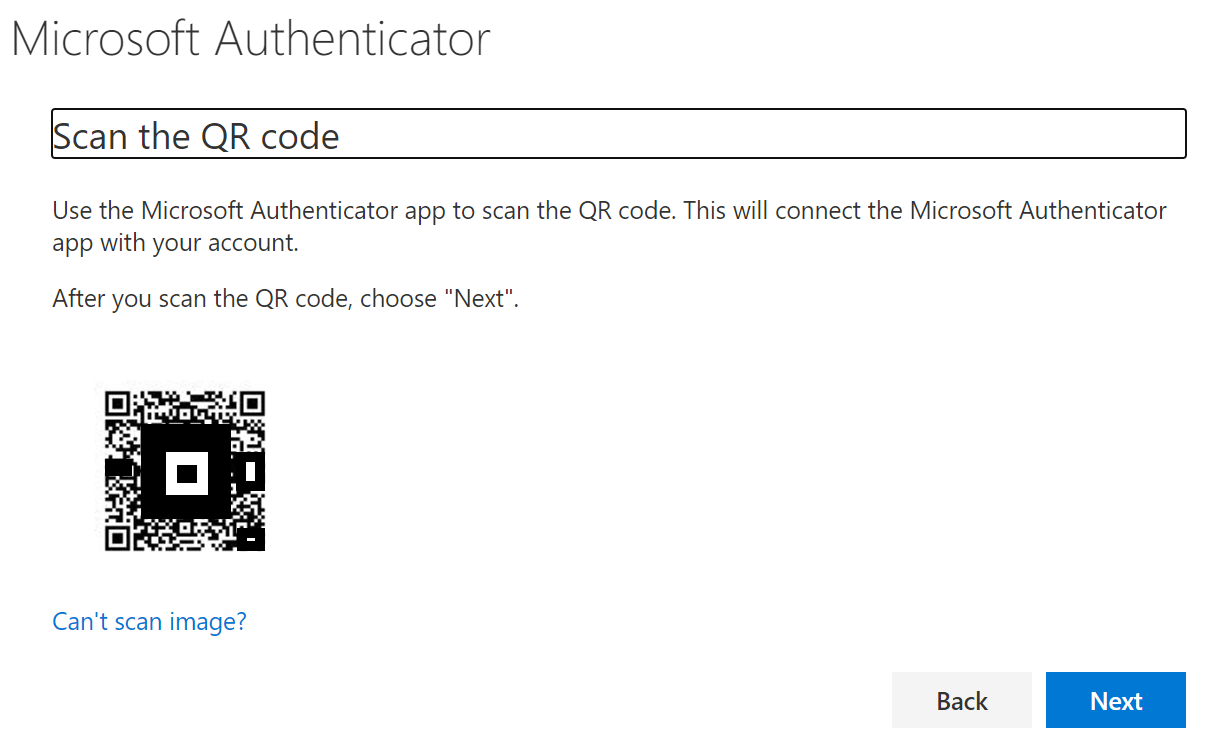
\includegraphics[width=1\textwidth]{./img/microsoft-auth-1.png}
		\end{figure}
			\begin{figure}
			\centering
			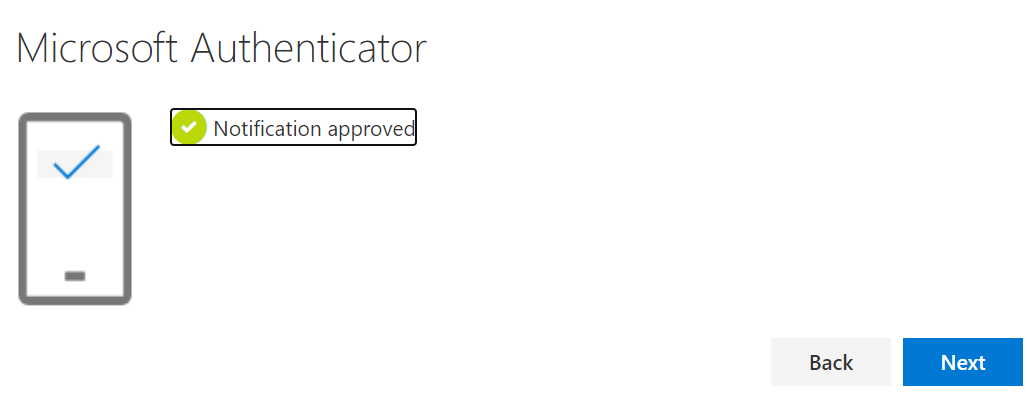
\includegraphics[width=1\textwidth]{./img/microsoft-auth-2.png}
		\end{figure}

	\end{columns}
\end{frame}

\begin{frame}
	\frametitle{WB AWS management console - log on}
	\begin{columns}[c]
		
		\column{.80\textwidth} % Right column and width
		
		\textbf{Log on:} The log on steps has to be done each time you access the AWS management console
		
	\end{columns}
\end{frame}

\begin{frame}
	\frametitle{WB AWS management console - log on}

	\begin{columns}[c]

		\column{.55\textwidth} % Right column and width

		When you are set up, this is how you access the AWS console each time:

		\begin{enumerate}
			\item Go to \url{cloudportal/} on WB intranet
			\item Log in using \textit{c$<$UPI$>$@worldbankgroup.org}
			(your C-account) and your new password
			\item Authenticate with \textit{Microsoft Authenticator}
			\item Click ``Amazon web service''
			\item Click ``AWS Account'', then expand (red square) and then click ``Management Console''

		\end{enumerate}

		\column{.45\textwidth} % Right column and width
		\begin{figure}
			\centering
			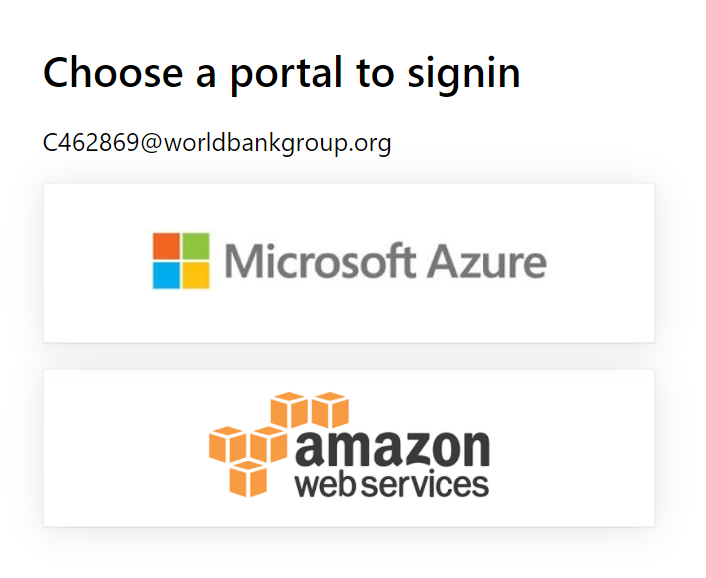
\includegraphics[width=.5\textwidth]{./img/logon-1.png}
		\end{figure}
		\vspace{.2cm}
		\begin{figure}
			\centering
			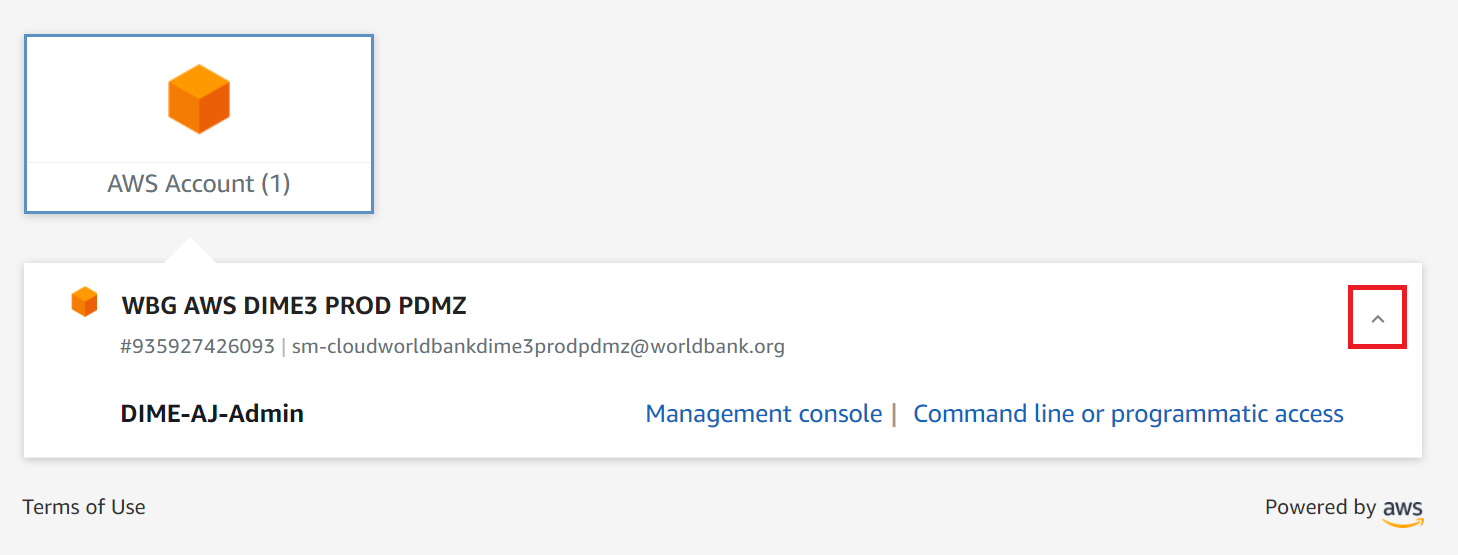
\includegraphics[width=1\textwidth]{./img/logon-2.png}
		\end{figure}
	\end{columns}
\end{frame}

\begin{frame}
	\frametitle{WB AWS management console - use case}
	\begin{columns}[c]
		
		\column{.80\textwidth} % Right column and width
		
		\textbf{Use cases:} This section has step-by-step guidelines for common tasks on the AWS management console
		
	\end{columns}
\end{frame}

\begin{frame}
	\frametitle{WB AWS management console - start an EC2 instance}

	\begin{columns}[c]

		\column{.60\textwidth} % Right column and width

			Start an EC2 instance (part 1 of 2):
	
			\begin{enumerate}
				\item In the AWS console, search for the service \textit{EC2} 
				\item To see the EC2 instances (servers), 
				click \textit{Instances} in the side menu - see top image to the right 
				\item Make sure that the you have selected region \textit{N. Virginia} (technical name: \texttt{us-east-1}) - see bottom image to the right. All WB AWS resources will be created in this region.
			\end{enumerate}


		\column{.40\textwidth} % Right column and width
			\begin{figure}
				\centering
				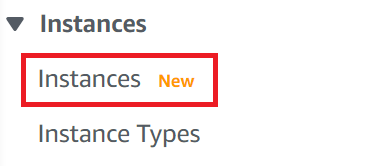
\includegraphics[width=.7\textwidth]{./img/ec2-1.png}
			\end{figure}		
			
			\begin{figure}
				\centering
				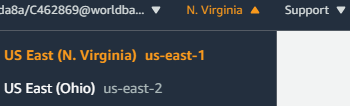
\includegraphics[width=.8\textwidth]{./img/aws-console-1.png}
			\end{figure}
	\end{columns}
\end{frame}


\begin{frame}
	\frametitle{WB AWS management console - start an EC2 instance}
	
	\begin{columns}[c]
		
		\column{.55\textwidth} % Right column and width
		
		Start an EC2 instance (part 2 of 2):
		
		\begin{enumerate}
			\setcounter{enumi}{3}
			\item Check the instance you want to start - for example \texttt{\ectwoName}
			\item Click \textit{Instance state} and select \textit{Start instance}
			\item Refresh until "Instance state" change from \textit{Pending} into \textit{Running}
		\end{enumerate}
		
		Your resource is now available to use. See next section for how to use it.

		\column{.45\textwidth} % Right column and width
		\begin{figure}
			\centering
			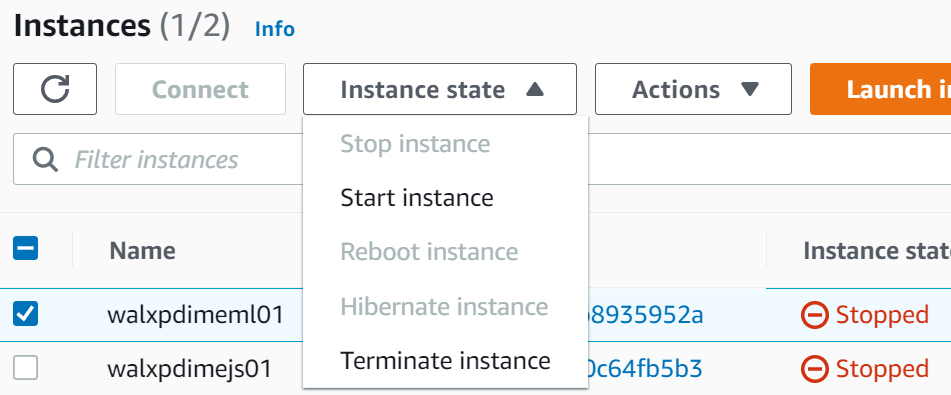
\includegraphics[width=1\textwidth]{./img/ec2-2.png}
		\end{figure}
		\begin{figure}
			\centering
			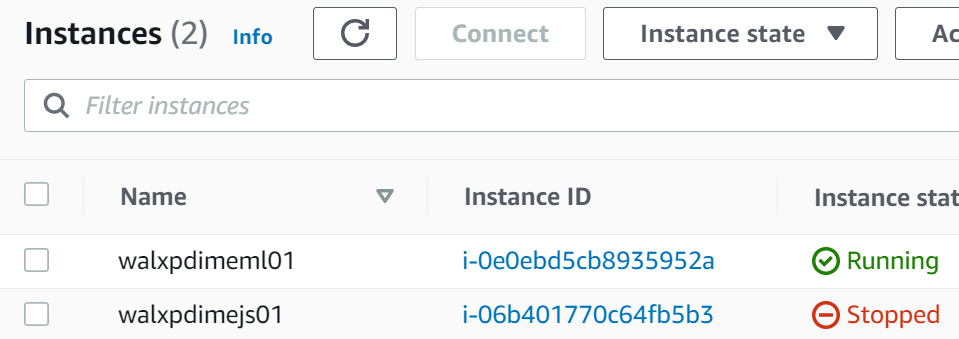
\includegraphics[width=1\textwidth]{./img/ec2-3.png}
		\end{figure}
		\vspace{.5cm}
		
	\end{columns}
\end{frame}

\section{Part 3: Command line access - WB AWS resources}

\begin{frame}
	\frametitle{Command line access - two types}

	Two ways to access an WB AWS resource, AWS cli or putty/ssh

	\vspace{.5cm}

	\begin{columns}[t]
		
		\column{.5\textwidth} % Left column and width
		\textbf{AWS cli (Part 3a):}
		\begin{itemize}
			%\setlength\itemsep{1em}
			\item Sends commands to the AWS API from the command line on your local computer
			\item You only see the output/errors that the API provides
			\item Not all API commands are allowed given WB AWS security settings
			\item Available om personal devices in some setups
		\end{itemize}
	
		\column{.55\textwidth} % Right column and width
		\textbf{Putty/ssh (Part 3b):}
		\begin{itemize}
			%\setlength\itemsep{1em}
			\item Connects by remotely logging you in to the instance
			\item Commands are executed directly on the instance and you see all output/errors in your terminal
			\item Can only be used on server type of resources, ex. EC2, but not on storage, ex. S3. (S3 can often be reached from EC2) 
		\end{itemize}
		
	\end{columns}
\end{frame}

\begin{frame}
	\frametitle{WB AWS command line access - CLI}
	\begin{columns}[c]
		
		\column{.80\textwidth} % Right column and width
		
		\textbf{Part 3a:} WB AWS command line access - CLI
		
	\end{columns}
\end{frame}

\begin{frame}
	\frametitle{WB AWS command line access - CLI - Security}
	\begin{columns}[c]
		\column{.60\textwidth} % Left column and width

		The AWS CLI authenticates the call to the API 
		using unique key pairs. 
		These key pairs must be treated with exceptional care as leaked keys can incur very big costs to the team.
		
		\vspace{.5cm} 
		
		AWS CLI keys may only be stored in 
		encrypted files or in a password manager, 
		or should be accessed each from 
		the AWS console each time needed.
		They should never be sent over email etc.
		
		\column{.45\textwidth} % Right column and width
		\begin{figure}
			\centering
			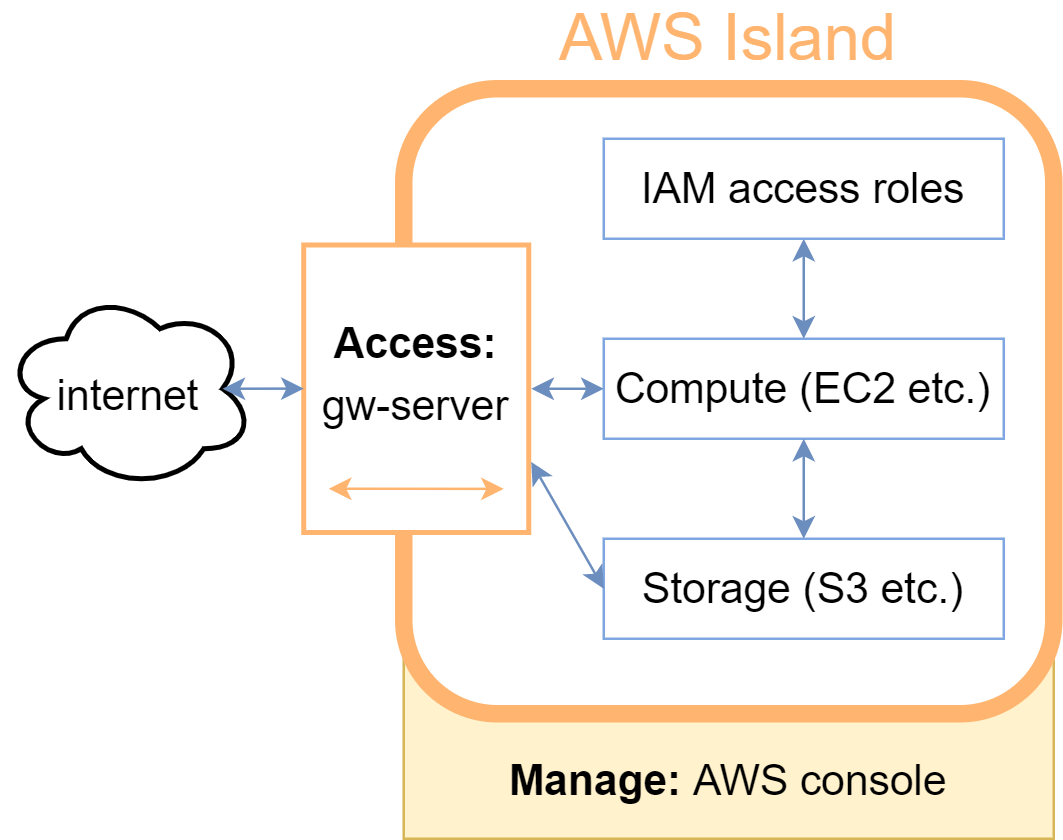
\includegraphics[width=\textwidth]{./img/wb-aws.png}
		\end{figure}
		
	\end{columns}
\end{frame}

\begin{frame}
	\frametitle{WB AWS command line access - CLI - Access keys}
	\begin{columns}[c]
		\column{.60\textwidth} % Left column and width

		Install the AWS CLI.
		\href{https://worldbankgroup.service-now.com/wbg?id=wbg_sc_catalog&sys_id=bd1e71b86f16d340db112d232e3ee4b7}{Request}
		for WB devices.
		\href{https://docs.aws.amazon.com/cli/latest/userguide/getting-started-install.html}{Guide} 
		for personal devices.

		\vspace{.5cm}

		Follow the steps in \textbf{Part 2} in this presentation
		to get to the view shown to the right.	
		Click \textit{Command line or programmatic access}.
		
		\vspace{.5cm} 
		
		There are multiple ways to configure the CLI, 
		this presentation uses Option 1. 
		Select your OS (red box).
		Click the code and save all of it in a password manager 
		(never email or unencrypted file) 
		or go to next slide to use immediately.
		
		\column{.45\textwidth} % Right column and width
		\begin{figure}
			\centering
			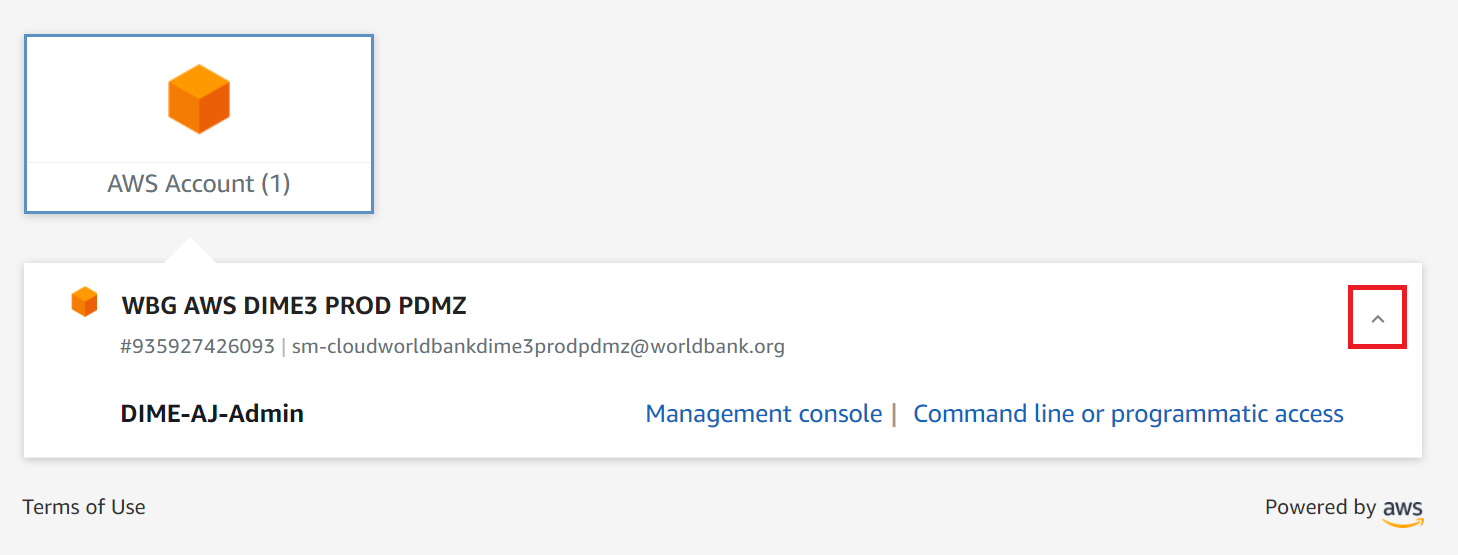
\includegraphics[width=1\textwidth]{./img/logon-2.png}
		\end{figure}
		\begin{figure}
			\centering
			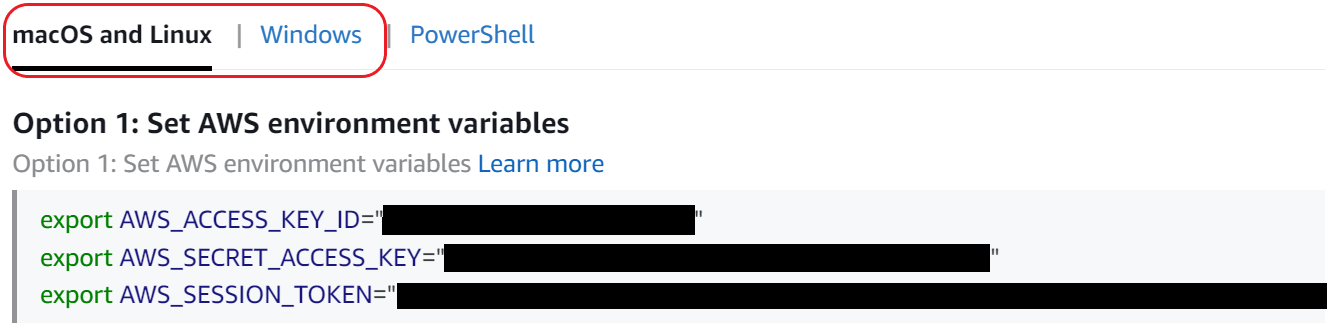
\includegraphics[width=1\textwidth]{./img/aws-cli-get-keys.png}
		\end{figure}
		
	\end{columns}
\end{frame}

\begin{frame}
	\frametitle{WB AWS command line access - CLI - Setup}
	\begin{columns}[c]
		\column{.60\textwidth} % Left column and width
		
		Open the command prompt or terminal where the AWS CLI was installed.
		
		\vspace{.5cm}
		
		Copy the full code from your password manager or from the AWS console if your just accessed the keys and paste to the command prompt or terminal. You paste with \textit{shift+insert} in command prompt. Hit enter.
		
		\vspace{.5cm} 
		
		Type \texttt{aws sts get-caller-identity} and hit enter to test access. Your configuration was successful if you see \texttt{UserID} and \texttt{Account} number.
		
		\column{.45\textwidth} % Right column and width
		\begin{figure}
			\centering
			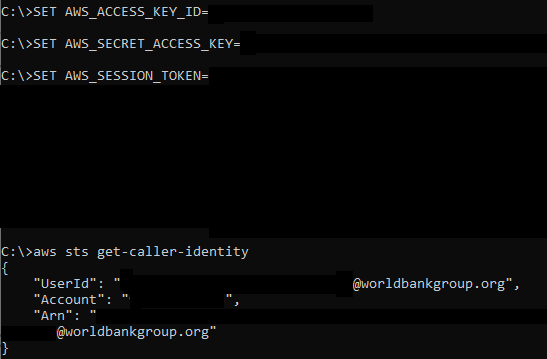
\includegraphics[width=1\textwidth]{./img/aws-cli-configure.png}
		\end{figure}
		
	\end{columns}
\end{frame}

\begin{frame}
	\frametitle{WB AWS command line access - CLI - Usage}
	\begin{columns}[c]
		\column{.60\textwidth} % Left column and width
		
		You can now start using the AWS CLI - see
		\url{https://docs.aws.amazon.com/cli/index.html}
		for documentation. 
		Not that not all actions available in the AWS CLI 
		are available on WB AWS resources.
		
		\vspace{.5cm}
		
		Your Access ID and Secret Access key do not expire
		but the Session Token might.
		If you suddenly lose access, 
		redo the setup in this presentation before
		reaching out to support.

		
		\column{.45\textwidth} % Right column and width
		\begin{figure}
			\centering
			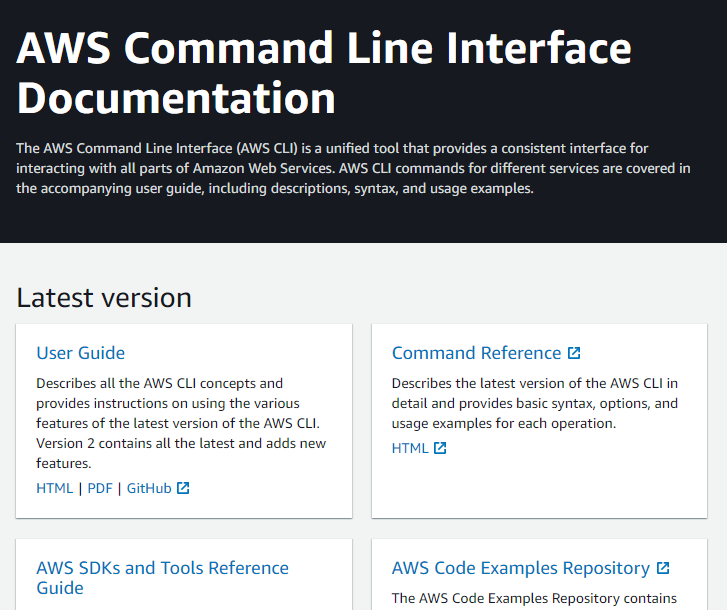
\includegraphics[width=1\textwidth]{./img/aws-cli-documentation.png}
		\end{figure}
		
	\end{columns}
\end{frame}

\begin{frame}
	\frametitle{WB AWS command line access - SSH}
	\begin{columns}[c]
		
		\column{.80\textwidth} % Right column and width
		
		\textbf{Part 3b:} WB AWS command line access - SSH
		
	\end{columns}
\end{frame}


\begin{frame}
	\frametitle{WB AWS command line access - SSH}
	\begin{columns}[c]
		\column{.60\textwidth} % Left column and width
		For resources that are a type of server - for example EC2 -
		you can remotely log to run scripts directly on the server. 
		
		\vspace{.5cm}
		
		This gives you the same access as if 
		you were physically connected to the machine, 
		meaning that you do connect over the API and 
		you see all output/errors that the resource returns.
		
		\vspace{.5cm}
		
		The process to set up a remote session using SSH
		might differ slightly depending on the resource.
		This guideline use the case of SSH into 
		an EC2 instance to, for example, run a script.

		\column{.45\textwidth} % Right column and width
		\begin{figure}
			\centering
			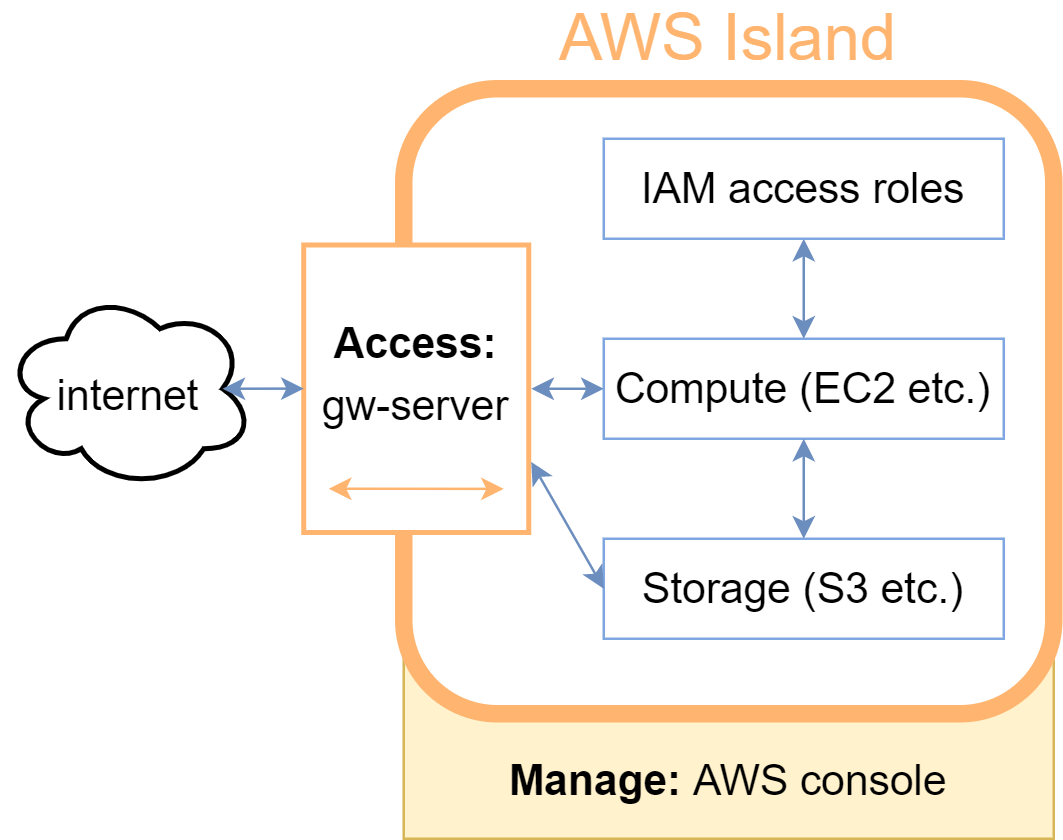
\includegraphics[width=\textwidth]{./img/wb-aws.png}
		\end{figure}

	\end{columns}
\end{frame}

\begin{frame}
	\frametitle{WB AWS command line access - SSH - PuTTY}
	\begin{columns}[c]
		\column{.60\textwidth} % Left column and width
		SSH is only available on WB devices
		(WB laptop/desktop or dedicated WB VDI)
		
		\vspace{.2cm}
		
		\begin{itemize}
			%\setlength\itemsep{1em}
			\item Make sure the EC2 instance is started
			(see \textbf{Part 2})
			\item Open PuTTY - self-install from 
			``\textit{Software Center}'' if needed
			\item Change ``\textit{Host name}''
			to either \textit{gw1}, \textit{gw2},
			\textit{gw3} or \textit{gw4}
			- \textit{gw} means ``\textit{gateway server}''. 
			Keep default values for all other settings.
			\item Click \textit{Open} 
		\end{itemize}

		\column{.4\textwidth} % Right column and width
		\begin{figure}
			\centering
			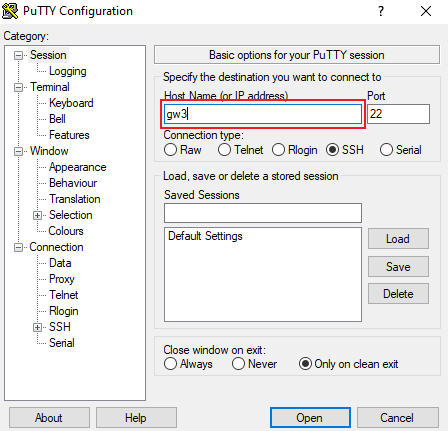
\includegraphics[width=\textwidth]{./img/access-1.png}
		\end{figure}

	\end{columns}
\end{frame}

\begin{frame}
	\frametitle{WB AWS command line access - SSH - Trust gw fingerprint}
	\begin{columns}[c]
		\column{.55\textwidth} % Left column and width
		\begin{itemize}
			\setlength\itemsep{1em}
			\item The first time you access each \textit{gw} server 
			you will get a warning that you have not 
			added that server to your trusted servers -
			see image to the right.
			\item Click \textit{Yes} and you will store this server's fingerprint (a unique ID).
			You will then not get this warning for this \textit{gw} server again
			unless the security of the connection is compromised.
		\end{itemize}
		
		\column{.45\textwidth} % Right column and width
		\begin{figure}
			\centering
			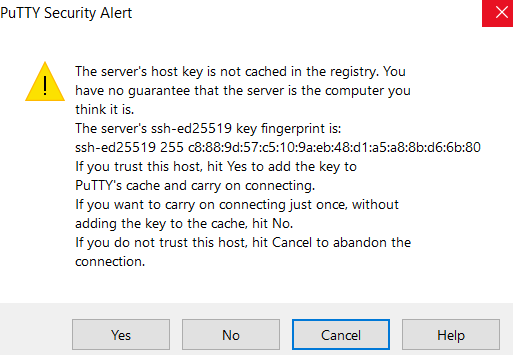
\includegraphics[width=\textwidth]{./img/access-1a.png}
		\end{figure}
		
	\end{columns}
\end{frame}


\begin{frame}
	\frametitle{WB AWS command line access - SSH - Authentication}
	\begin{columns}[c]
		\column{.50\textwidth} % Left column and width
		\begin{itemize}
			%\setlength\itemsep{1em}
			\item Enter your UPI on format \texttt{wb$<$UPI$>$} - press \textit{Enter}
			\item Open your SecureID and enter token for \textit{First Factor} - press \textit{Enter}
			\item Leave \textit{Second Factor} empty - just press \textit{Enter}
			\item This step was successful if your prompt says:
			\texttt{wb<yourUPI>@w01xidmgw3}
			- (gw3 depends on which gw server you chose)
		\end{itemize}

		\column{.55\textwidth} % Right column and width
		\begin{figure}
			\centering
			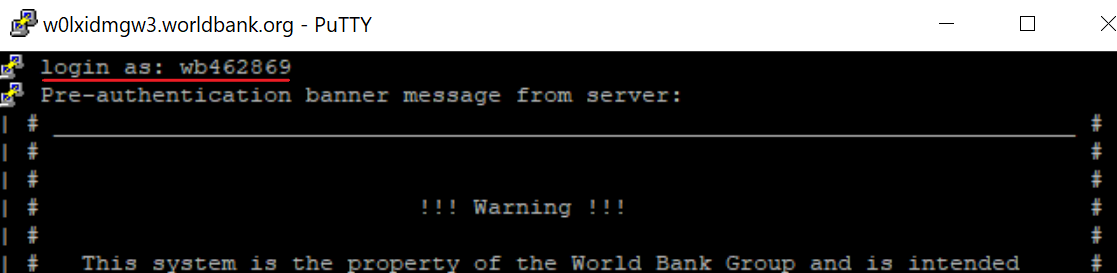
\includegraphics[width=\textwidth]{./img/access-2a.png}
			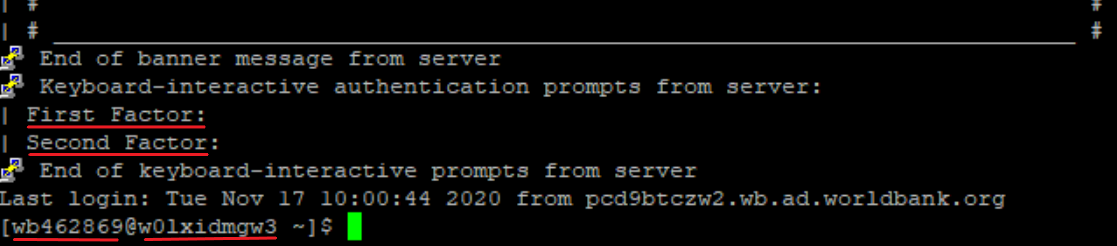
\includegraphics[width=\textwidth]{./img/access-2b.png}
		\end{figure}

	\end{columns}
\end{frame}

\begin{frame}
	\frametitle{WB AWS command line access - SSH - SHH to your instance}
	\begin{columns}[c]
		\column{.50\textwidth} % Left column and width
		\begin{itemize}
			%\setlength\itemsep{1em}
			\item You are now authenticated in the WB AWS Island
			\item Connect to your EC2 instance by typing: \newline
			\texttt{ssh \textit{instance-name}}. 
			Replace \textit{instance-name} with the name 
			ITS provided your team with.
			\item This step was successful if your prompt says:
			\texttt{wb<yourUPI>@<instance-name>}
		\end{itemize}

		\column{.55\textwidth} % Right column and width
		\begin{figure}
			\centering
			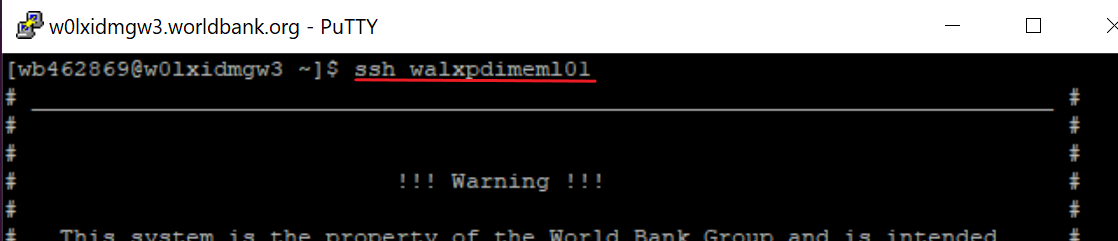
\includegraphics[width=\textwidth]{./img/access-3a.png}
			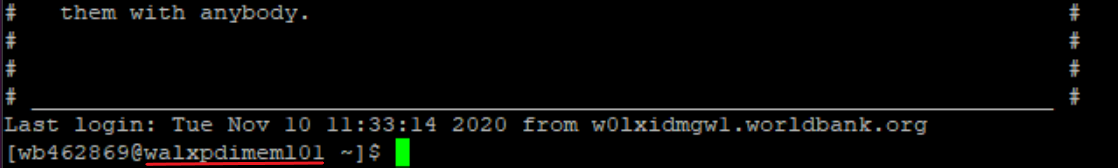
\includegraphics[width=\textwidth]{./img/access-3b.png}
		\end{figure}

	\end{columns}
\end{frame}

\begin{frame}
	\frametitle{WB AWS command line access - SSH - assume team role}
	\begin{columns}[c]
		\column{.55\textwidth} % Left column and width
		\begin{itemize}
			%\setlength\itemsep{1em}
			\item Access to anything meaningful are only given to  team's "service accounts", not to individual accounts
			\item Assume your team's service account by typing: \newline
			\texttt{sudo su - \textit{service-account-name}}. Replace \textit{service-account-name} with the name 
			ITS provided your team with.
			\item This step was successful if 
			your prompt says:
			\newline\texttt{<service-account-name>@<instance-name>}
		\end{itemize}

		\column{.50\textwidth} % Right column and width
		\begin{figure}
			\centering
			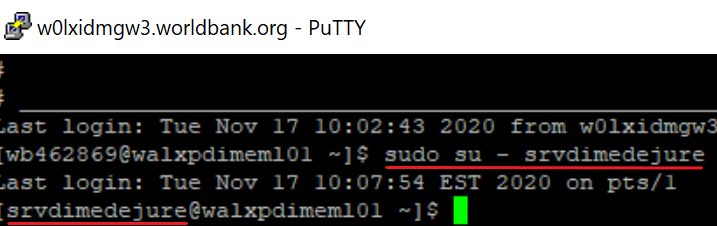
\includegraphics[width=\textwidth]{./img/access-4.png}
		\end{figure}

	\end{columns}
\end{frame}

\begin{frame}
	\frametitle{WB AWS command line access - SSH - run a script}
	\vspace{1cm}
	\begin{columns}[c]
		\column{.5\textwidth} % Left column and width
		You may now run scripts on the EC2 instance. 
		
		\vspace{.5cm}
		
		Remember that no matter what OS you use
		on your local machine, 
		you may only use Linux terminal on EC2 instances.
		See next slide for a cheat sheet to Linux terminal commands.
		
		\column{.55\textwidth} % Right column and width
		\begin{figure}
			\centering
			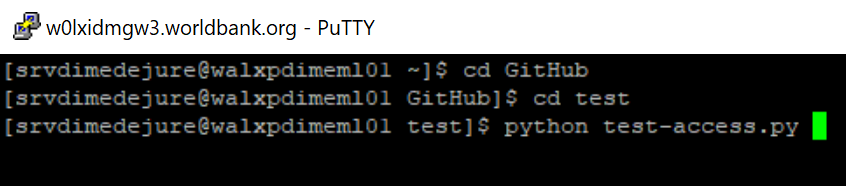
\includegraphics[width=\textwidth]{./img/access-5.png}
		\end{figure}
	\end{columns}
\end{frame}

\begin{frame}
	\frametitle{Linux commands - cheat sheet}
	\vspace{-.6cm}
	\begin{table}
		\begin{tabular}{p{0.355\textwidth}p{0.62\textwidth}}
			Command & Function \\
			\hline \hline
			\texttt{cd \textit{filepath}}
			  & Change working directory to \textit{filepath}  \\
			\texttt{cd $\sim$}
			  & Change working directory to \textit{home}/\textit{user} directory \\
			\texttt{cd ..}
			  & Change working directory to the parent folder of current working directory \\
			\texttt{mv \textit{oldpath} \textit{newpath}}
			  & Move a file or folder, can also be used to rename a file or folder \\
			\texttt{vim \textit{filename}}
			  & Opens a very basic code editor on the EC2 instance \\
			\texttt{python \textit{filename.py}}
			  & Run python scripts with name \textit{filename.py} \\
			\texttt{git clone \textit{repo-clone-url}}
			  & Clones repo to EC2 instance (find clone URL on GitHub) \\
			\texttt{git checkout \textit{branch}}
			  & Switch to branch in the clone\\
			\texttt{git pull}
			  & Download new edits in the branch  \\
		\end{tabular}
	\end{table}
\end{frame}

\begin{frame}
	\frametitle{Thank you!}

	\begin{columns}[c]

		\column{.10\textwidth} % Left column and width

		\column{.35\textwidth} % Left column and width
		\Huge Thank you!

		\vspace{1cm}

		\Huge Questions?

		\column{.45\textwidth} % Right column and width
		\begin{figure}
			\centering
			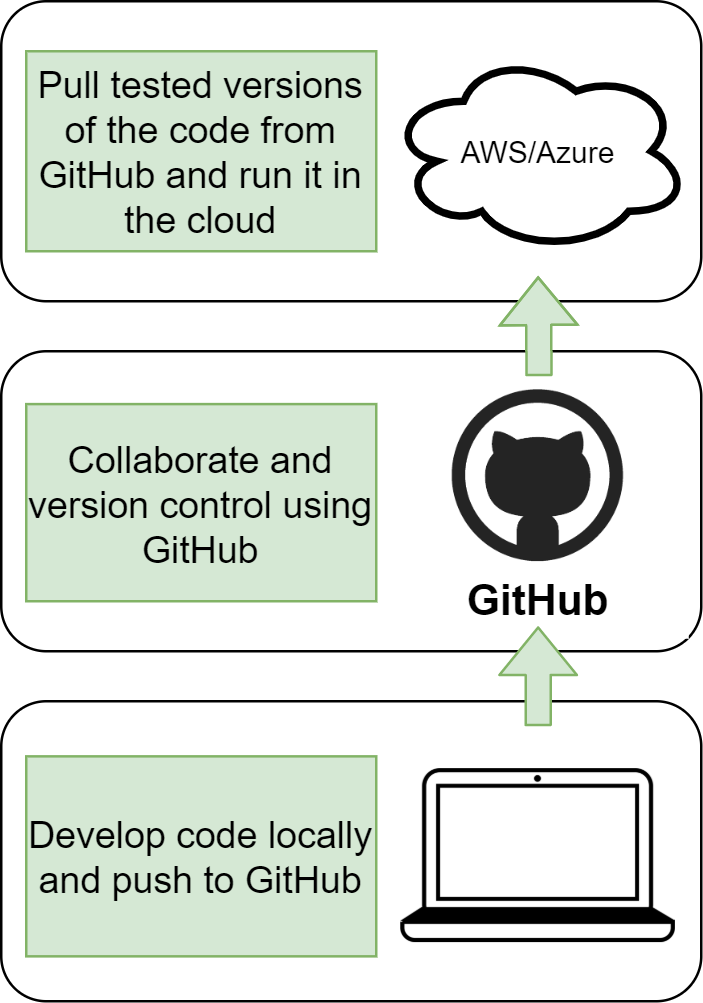
\includegraphics[width=.7\textwidth]{./img/code-workflow.png}
		\end{figure}

		\column{.10\textwidth} % Left column and width
	\end{columns}
\end{frame}

\end{document}
